\documentclass[12pt, preprint,letterpaper]{article}
\usepackage{epsfig}
\usepackage{xspace}
\usepackage{amsmath}
\usepackage{mathrsfs}
\usepackage{xcolor}
\usepackage{graphicx}
\usepackage{cite}
\usepackage{natbib}
\usepackage{hyperref}
\usepackage[utf8]{inputenc}
\graphicspath{ {figures/} }
%%for list of tables
\usepackage{etoolbox}
\makeatletter
\patchcmd{\@caption}{\csname the#1\endcsname}{\csname fnum@#1\endcsname:}{}{}
\renewcommand*\l@figure{\@dottedtocline{1}{1.5em}{4.5em}} % default for 3rd arg: 2.3em
\let\l@table\l@figure % as in article.cls
\makeatother
%% end list of tables
%%
% Begin of document
\begin{document}
%
%
%#******************************************************************************
%#==============================================================================
%#          Beginning: Preamble page
%#==============================================================================
%#******************************************************************************
%
\thispagestyle{empty}
\begin{center}
\textbf{Effects of Wavelenth Dependence on Galaxy Shear Measurement} \\

\vspace{2cm}
PH.D. THESIS PROSPECTUS BY BHISHAN POUDEL \\
(ADVISOR: ASSOCIATE PROF. DOUGLAS CLOWE) \\

\vspace{3cm}
\it{
Department of Physics and Astronomy\\
Ohio University\\
Athens, OH 45701\\
\vspace{2cm}
bp959314@ohio.edu\\
}


\vspace{3cm}
\it{
Prof. Douglas Clowe\,  \hspace{2mm} (Department of Physics \& Astronomy)\\
Prof. Ryan Chornock\,  \hspace{2mm} (Department of Physics \& Astronomy)\\
Prof. Hee Jong Seo\, \hspace{3mm} (Department of Physics \& Astronomy)
}

\end{center}
%
%
%#******************************************************************************
%#==============================================================================
%#          Table of contents
%#==============================================================================
%#******************************************************************************
%
%
\clearpage
\tableofcontents
\listoffigures 
\listoftables
\clearpage{}
%
%
%#******************************************************************************
%#==============================================================================
%#          List of Acronyms
%#==============================================================================
%#******************************************************************************
%
\thispagestyle{empty}
\begin{center}
\textbf{LIST OF ACRONYMS}
\end{center}
\textbf{CDM}    \hspace{9.5mm} Cold Dark Matter \\
\textbf{CMB}    \hspace{10mm} Cosmic Microwave Background \\
\textbf{DE}     \hspace{15mm} Dark Energy \\
\textbf{DM}     \hspace{14mm} Dark Matter \\
\textbf{FWHM}   \hspace{6mm} Full Width Half Maximum \\
\textbf{GR}     \hspace{15mm} General Relativity \\
\textbf{HST}    \hspace{13mm} Hubble Space Telescope \\
\textbf{IMCAT}  \hspace{7mm} Image and Catalogue Manipulation Software \\
\textbf{LSS}    \hspace{15mm} Large Scale Structure \\
\textbf{LSST}   \hspace{12mm} Large Synoptic Survey Telescope \\
\textbf{PSF}    \hspace{14mm} Point Spread Function \\
\textbf{SED}    \hspace{14mm} Spectral Energy Distribution \\
\textbf{WFIRST} \hspace{4mm}  Wide-Field Infrared Survey Telescope \\
%longest word wfirst is 6 letter long and make it 4mm wide.
%one letter less is about 3mm longer space.

\newpage
%
%
%#******************************************************************************
%#==============================================================================
%#          Section 1: Introduction
%#==============================================================================
%#******************************************************************************
%
%
\section{Introduction}\label{sec:sec1}
According to standard model of cosmology dark matter accounts for  28.5\% of total mass energy content of the Universe.  
It's mainly dominated in Galaxy and Galaxy Clusters.  
Anisotropy in the Cosmic microwave background,cosmic 
structure formation,galaxy formation
and evolution suggest the presence of dark matter.  
As it does not interact with electromagnetic radiation and 
visible matter the method it can  be detected is by observing 
it's effect on ordinary baryonic matter.  
Gravitational Lensing provides us a way
to see how dark matter along with visible matter is distributed 
in a galaxy or galaxy cluster.  
This is supported by Einstein's general theory of relativity 
which predicts the deflection of light in a gravitational field 
produced by a massive object. (refer to \cite{fabian12})

%
%
%#------------------------------------------------------------------------------
%#          Subsection 1a: 
%#------------------------------------------------------------------------------
%
%
\subsection{subsection1: Formulation of Gravitational Lensing}\label{subsec:}
Gravitational Lensing provides us a way
to see how dark matter along with visible matter is distributed 
in a galaxy or galaxy cluster.  
This is supported by Einstein's general theory of relativity 
which predicts the deflection of light in a gravitational field 
produced by a massive object. (refer to \cite{fabian12})
%
%
%#******************************************************************************
%#==============================================================================
%#          Section 2:  Future Projects
%#==============================================================================
%#******************************************************************************
%
%
\section{Future Projects}\label{sec:sec2}
 \begin{figure}[h!]
 \centering
  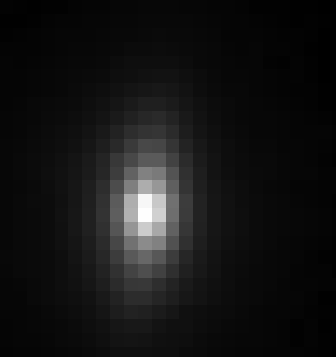
\includegraphics[width=0.5\textwidth]{convolve.png}
 \caption{This is caption.}
 \end{figure}
\newpage{}
%
%
%#******************************************************************************
%#==============================================================================
%#          Section 3: Timeline
%#==============================================================================
%#******************************************************************************
%
%
\section{Timeline}
I intend to complete all elements of this project within two years. 
An outline of the projected time line is presented in the table below. 
The dates and activities displayed are subject to change should
unforeseen and interesting developments occur during the projects that 
may require special attention and time.
\begin{table}[h]
\caption{Timeline}
\vspace{5mm}
\centering
        \begin{tabular}{|c|c|c|}
            \hline
            Start&Finish&Activity\\
            \hline
            Sep. 2016& March 2017 &  \\
            \hline
            April 2017 & Sep. 2017 &   \\
            \hline
            Sep. 2017 & March 2018 & Preparation of manuscripts for publication \\
            \hline
            March 2018 & Aug. 2018& Writing and defending the dissertation   \\
            \hline
            \end{tabular}
\end{table}
%
%
%#******************************************************************************
%#==============================================================================
%#               Bibliography and End Document
%#==============================================================================
%#******************************************************************************
%
%
\newpage
\bibliographystyle{plain}
\bibliography{bib/prospectus}
\end{document}
